\section{CCMP Agent Framework}
The ART testbed provides a base Agent class with several functions that must be
implemented by the new agent. These functions allow the agent to interact with
the other agents and participate in the game through the exchange of differet
messages.  

To facilitate the distributed development environment it was important to break
the agent environment into different parts.  The CCMP Agent consists of the
base CCMP Agent class, base Trust Network interface class, an base Decision
Tree interface class and their associated implementations.

\subsection{Main Agent}
The base framework class, CCMPAgent, is the subclass of the ART testbed Agent
and provides the interface to the ART testbed.  The CCMPAgent is
responsible for handling the generation, parsing and responses to the
messages within the testbed Agent methods.  

It does this in a similar and abstact manner for each one. First it parses the
incoming messages and updates the trust network and decision tree on the
results of the messages, either positive or negative.  After updating the
knowledge base regarding the actions of the other agents and passing the new
values from the trust network to the decision tree if queries the decision tree
to determine what action to take.  It then generates the appropriate
messages and passes them to the sim.

The base CCMPAgent class implements all this functionality in an abstract way
using the base TrustNetwork and DecisionTree classes.  The specific objects
types, such as the Bayesian trust network and Weka decision tree, are
instantiated in subclasses of CCMPAgent.  It is these subclasses that are passed
to the ART testbed for creation in the sim.  In this manner different
implementations of the trust network and decision tree classes can be easily
incorperated into the CCMPAgent.

\begin{center}
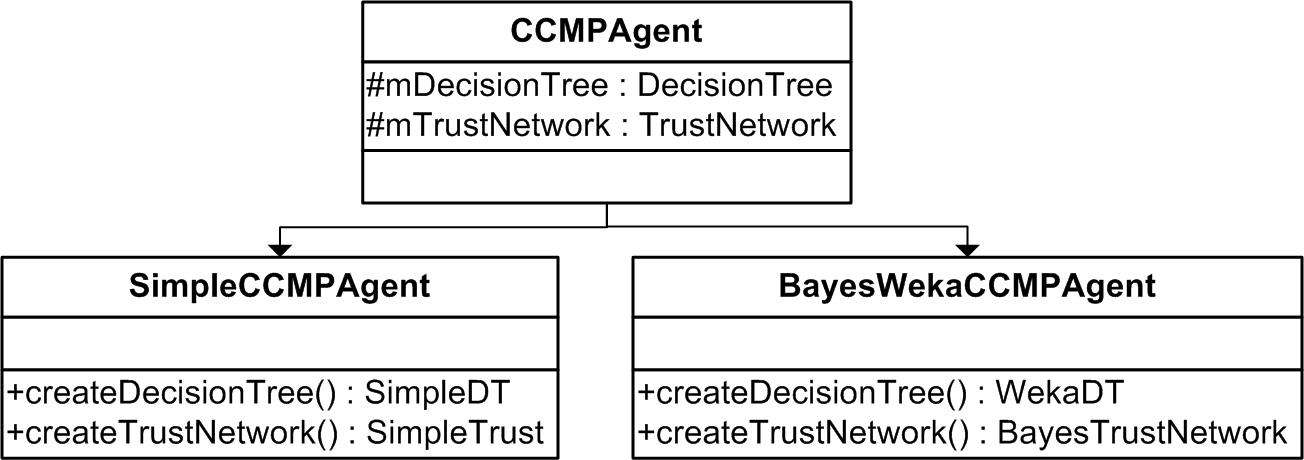
\includegraphics{images/CCMPClasses.jpg}
\end{center}

\subsection{Trust Network}
The trust network is an abstract class used to represent the trust the agent
has for other players.  The interface class provides methods to update the
trust values based on events in the sim, such as receiving new reputation
information from other agents or negative actions by an agent.  At the end of
each frame the resulting final appraisal and each agents opinion are also
passed to the trust network as they could be used to update trust values.

The trust network also allows for the representation of inferred trust, or the
trust we believe an other agent has for us.  This value could be used by the
decision tree to affect decisions and can be modelled both by asking the other
agent about our reputation and by keeping track of our actions to the specific
agent.  To this end several methods are provided that will tell the trust
network about the actions the CCMPAgent has taken, such as not providing the
requested information or modifying the appraisal value.

\begin{center}
\begin{array}{cc}
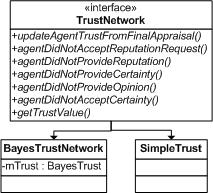
\includegraphics{images/TrustNetworkClasses.jpg} &
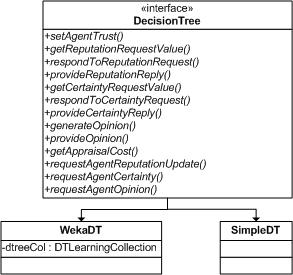
\includegraphics{images/DTClasses.jpg}
\end{array}
\end{center}

\subsection{Decision Tree}
Abstract class that provides direction to the agent on how to behave.  For each
possible action (list actions) the DT has a function to provide direction to
the main agent class.
